\begin{comment}
\begin{titlepage}
\begin{center}
 \Huge \textbf{\textsc{Solutions}}\\[1cm]
 \Huge \textbf{\textsc{Electronics \& Signal Processing}}\\[1cm]
 \Huge \textbf{\textsc{Chapter 3}}\\[3cm]
 \LARGE M BMTP / BS P \& A \\[1cm]
\Large


\begin{figure}[b]
\center{
\includegraphics[width = 150mm]{Figures/logoVUvA}}			
\end{figure}

\end{center}
\end{titlepage}
\end{comment}

\chapter{DC circuits}

\section{\textbf{Exercise 3.1}}
\noindent (a) \\
Since there is no load between terminals $a$ and $b$ $V_{\rm Th}$ does not depend on the $3k3$ loads. $V_{\rm Th}$ is given by (see Fig. \ref{fig:31a1}a):
\begin{center}
    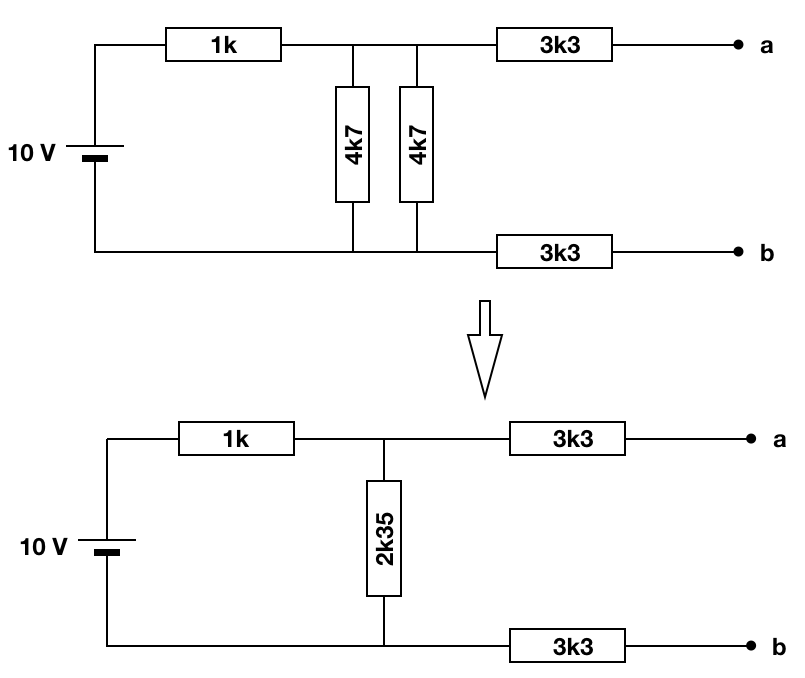
\includegraphics[width=0.8\textwidth]{Figures/31a1} 

    Figure 3.1a: Determination of $V_{\rm Th}$	  
    \label{fig:31a1} 
\end{center} 


\begin{equation}
V_{\rm Th} = \frac{2k35}{1k + 2k35} \cdot 10 = 7 V.
\end{equation}

\newpage
\noindent To calculate $R_{\rm Th}$ the voltage source should be removed (see Fig. \ref{fig:31a2}b):
\begin{center}
    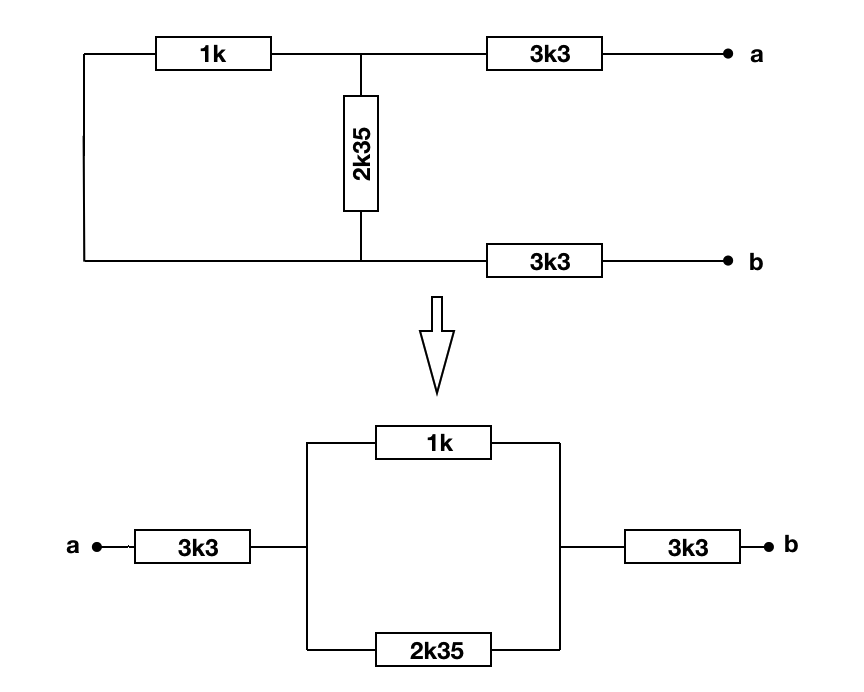
\includegraphics[width=0.8\textwidth]{Figures/31a2}	
    
    Figure 3.1b: Determination of $R_{\rm Th}$	  
\label{fig:31a2} 
\end{center}

\begin{equation}
R_{\rm Th} = 2 \cdot 3k3 + (1k || 2k35) = 7k3.
\end{equation}

\noindent This results in Fig. \ref{fig:31a3}c.
\begin{center}
    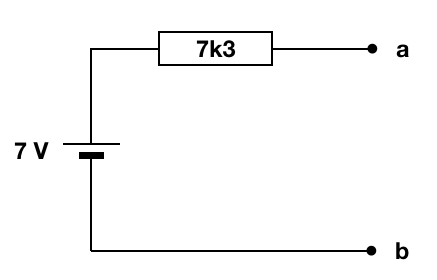
\includegraphics[width=0.5\textwidth]{Figures/31a3}	
 
    Figure 3.1c: Th\'{e}venin equivalent circuit	  
    \label{fig:31a3} 
\end{center}

\newpage
\noindent The result in Multisim is the same (see Fig. \ref{fig:31aM}d):
\begin{center}
    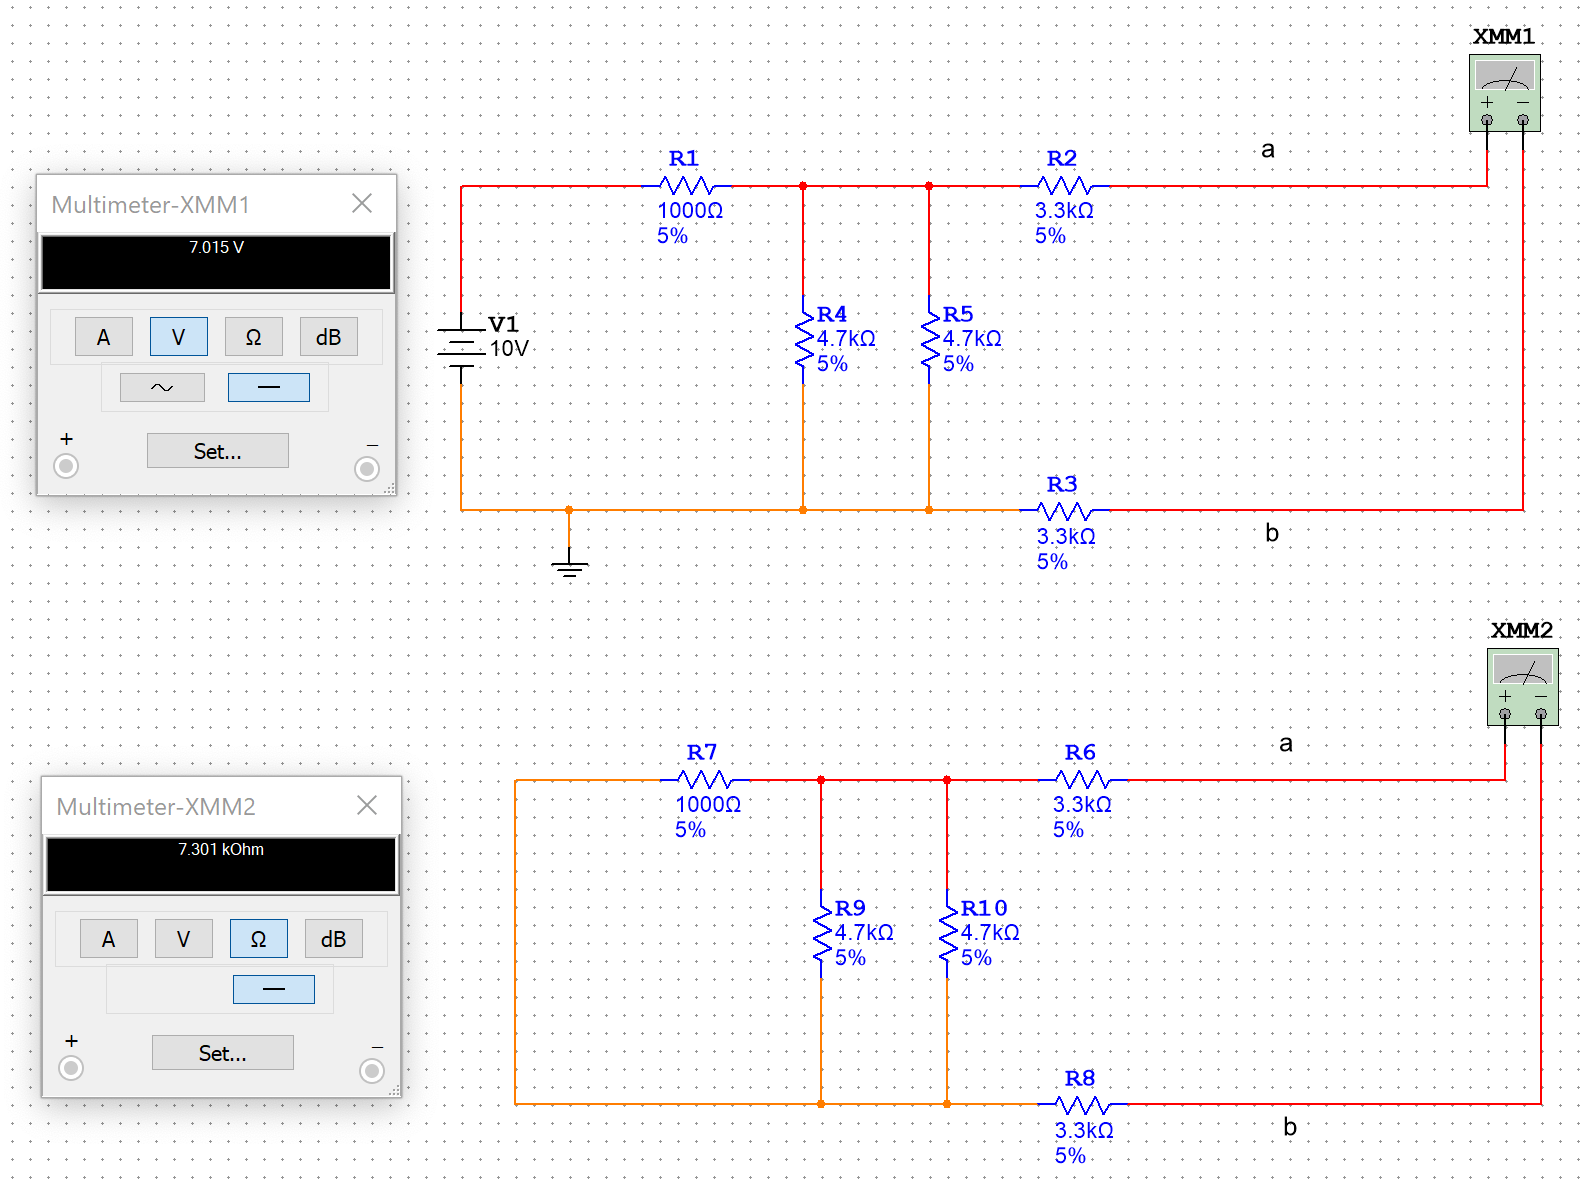
\includegraphics[width=1.0\textwidth]{Figures/31aMulti}	
 
    Figure 3.1d: The results of \textit{Mult 3.1a}	  
    \label{fig:31aM} 
\end{center}

\noindent (b) \\
To determine $V_{\rm Th}$ you first need to determine $I_{\rm Th}$ (see Fig. \ref{fig:31b1}e):
\begin{center}
    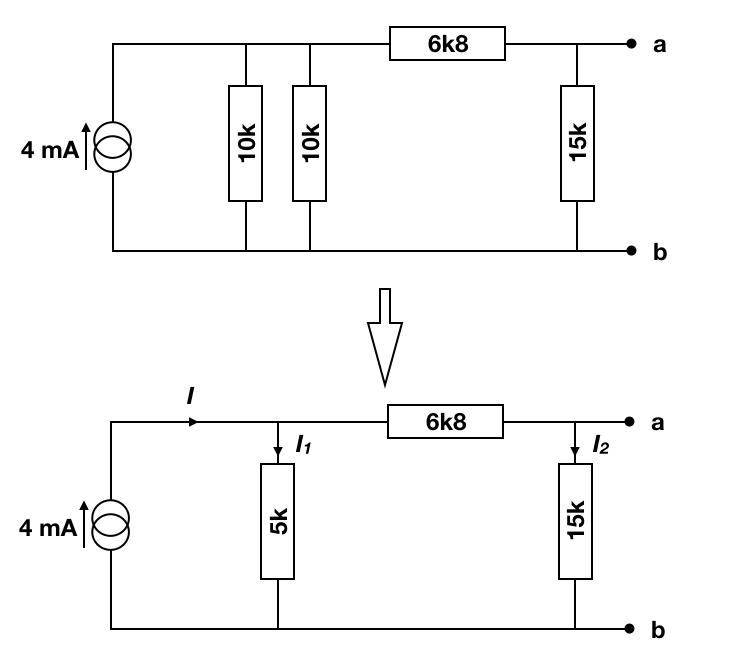
\includegraphics[width=0.7\textwidth]{Figures/31b1}	
 
    Figure 3.1e: Determination of $V_{\rm Th}$	  
    \label{fig:31b1} 
\end{center}

\begin{equation}
\begin{split}
V_{\rm Th} = I_2 \cdot 15k \\
I = I_1 + I_2 \\
\sum V_{\rm Closed \; Loop} = 0 \\
I_1 \cdot 5k - I_2 \cdot (6k8 + 15k) = 0 \\
(I - I_2) \cdot 5k - I_2 \cdot (6k8 + 15k) = 0 \\
I \cdot 5k - I_2 \cdot 26k8 = 0 \\
I_2 = \frac{4 \; {\rm mA} \cdot 5k}{26k8} = 0.75 \; {\rm mA}. \\
V_{\rm Th} = 0.75 \; {\rm mA} \cdot 15k \; \Omega = 11.2 \; {\rm V}.
\end{split}
\end{equation}
 
\noindent To determine $R_{\rm Th}$ the current source should be removed by open terminals (see Fig. \ref{fig:31b2}f), 
\begin{center}
    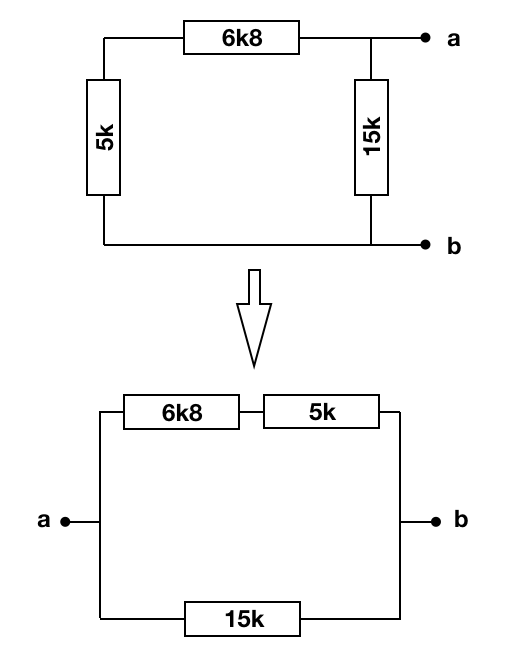
\includegraphics[width=0.5\textwidth]{Figures/31b2}	
 
    Figure 3.1f: Determination of $R_{\rm Th}$	  
    \label{fig:31b2} 
\end{center}

\noindent so:
\begin{equation}
R_{\rm Th} = (6k8 +5k || 15k) = 6k6.
\end{equation}
 
\newpage
\noindent This results in Fig. \ref{fig:31b3}g.
\begin{center}
    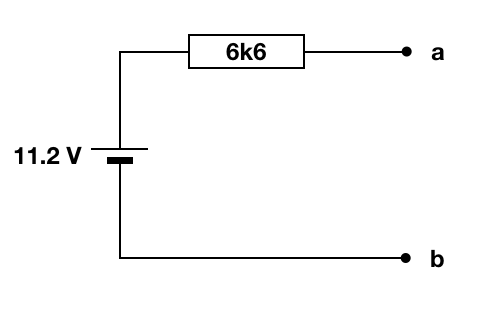
\includegraphics[width=0.5\textwidth]{Figures/31b3}	
 
    Figure 3.1g: Th\'{e}venin equivalent circuit	  
    \label{fig:31b3} 
\end{center}

\noindent The result in Multisim is the same (see Fig. \ref{fig:31bM}h):
\begin{center}
    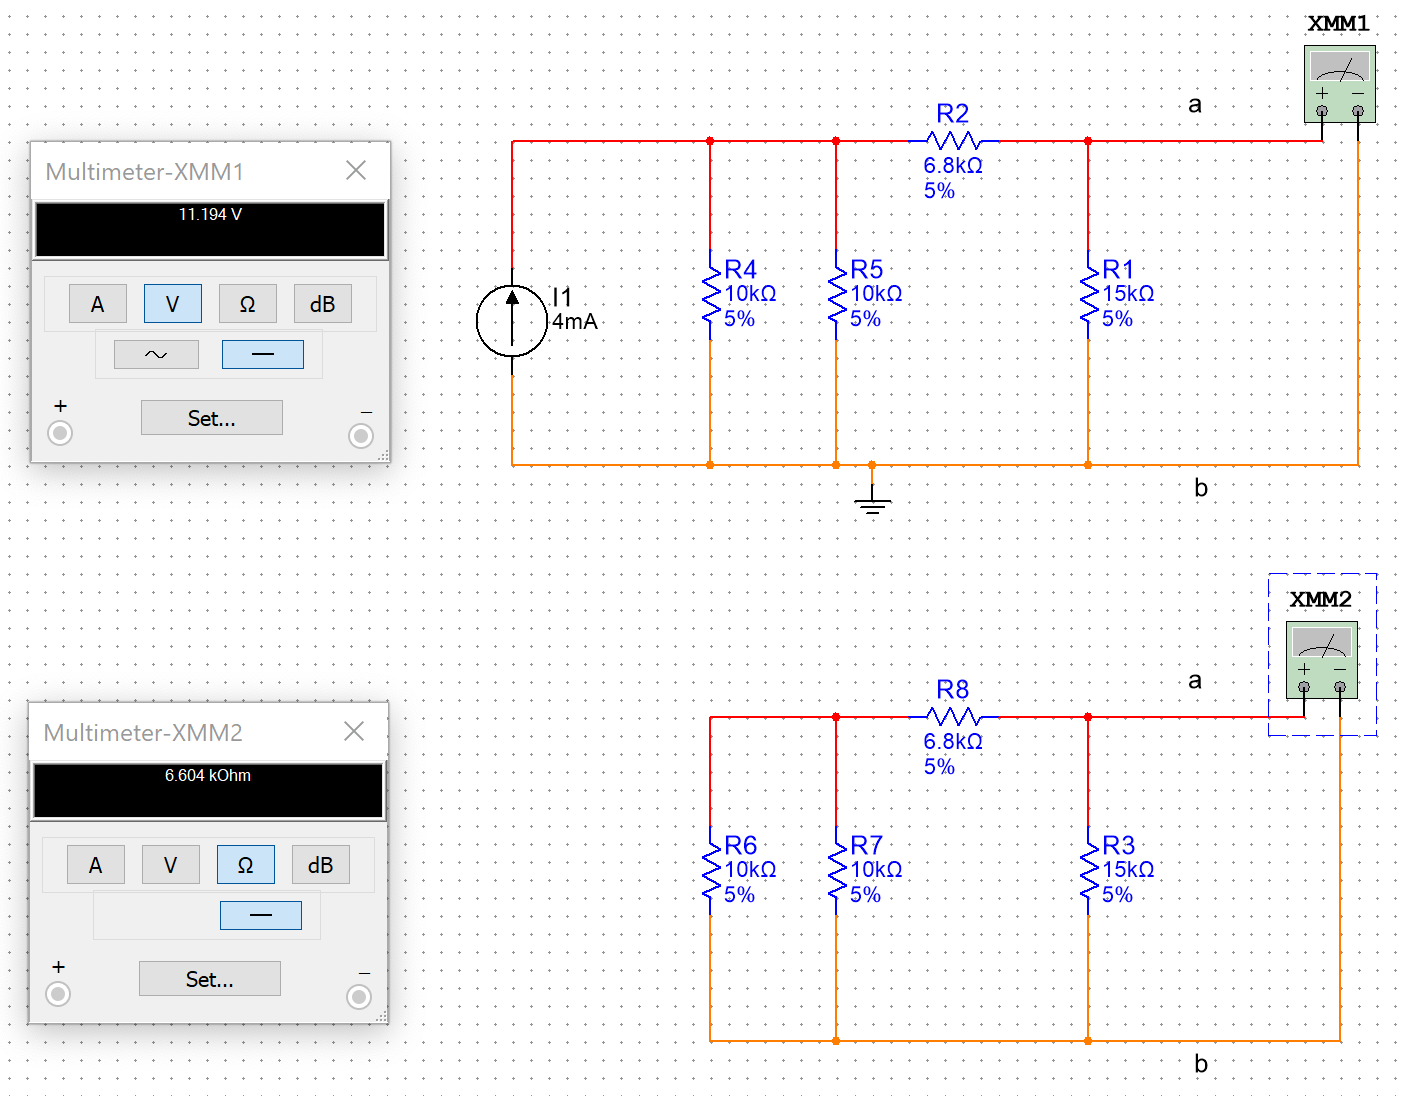
\includegraphics[width=1.0\textwidth]{Figures/31bMulti}	
 
    Figure 3.1h: The results of \textit{Mult 3.1b}	  
    \label{fig:31bM} 
\end{center}

\newpage
\section{\textbf{Exercise 3.2}}
In order to determine $V_{\rm Th}$ the circuit needs to be split up into two circuits with one current source each (see Fig. \ref{fig:32-1}a). 
\begin{center}
    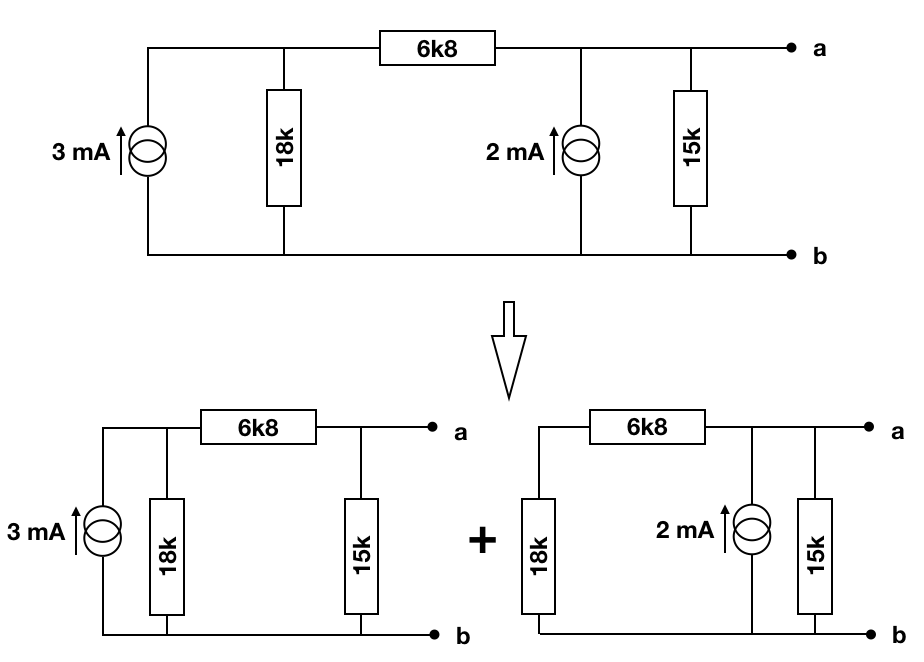
\includegraphics[width=0.7\textwidth]{Figures/32-1}
 
    Figure 3.2a: Determination of $V_{\rm Th}^{\rm 3 \; mA}$ and $V_{\rm Th}^{\rm 2 \; mA}$	  
    \label{fig:32-1} 
\end{center}

\noindent Then the $V_{\rm Th}$ can be determined for each circuit.
\begin{equation}
\begin{split}
V_{\rm Th}^{\rm 3 mA} = I_2 \cdot 15k \\
I = I_1 + I_2 \\
\sum V_{\rm Closed \; Loop} = 0 \\
I_1 \cdot 18k - I_2 \cdot (6k8 + 15k) = 0 \\
(I - I_2) \cdot 18k - I_2 \cdot (6k8 + 15k) = 0 \\
I \cdot 18k - I_2 \cdot 39k8 = 0 \\
I_2 = \frac{3 \; {\rm mA} \cdot 18k}{39k8} = 1.36 \; {\rm mA}. \\
V_{\rm Th}^{\rm 2 \; mA} = 1.36 \; {\rm mA} \cdot 15k \; \Omega = 20.35 \; {\rm V}.
\end{split}
\end{equation}
\begin{equation}
\begin{split}
V_{\rm Th}^{\rm 2 mA} = I_2 \cdot 15k \\
I = I_1 + I_2 \\
\sum V_{\rm Closed \; Loop} = 0 \\
I_1 \cdot (6k8 + 18k) - I_2 \cdot 15k = 0 \\
(I - I_2) \cdot (6k8 + 18k) - I_2 \cdot 15k = 0 \\
I \cdot 24k8 - I_2 \cdot 39k8 = 0 \\
I_2 = \frac{2 \; {\rm mA} \cdot 24k8}{39k8} = 1.25 \; {\rm mA}. \\
V_{\rm Th}^{\rm 2 \; mA} = 1.25 \; {\rm mA} \cdot 15k \; \Omega = 18.69 \; {\rm V}.
\end{split}
\end{equation}
So $V_{\rm Th}$ is
\begin{equation}
V_{\rm Th} = 20.35 + 18.69 = 39.04 V.
\end{equation}

To determine $R_{\rm Th}$ the current sources should be removed by open terminals (see Fig. \ref{fig:32-2}b), 
\begin{center}
    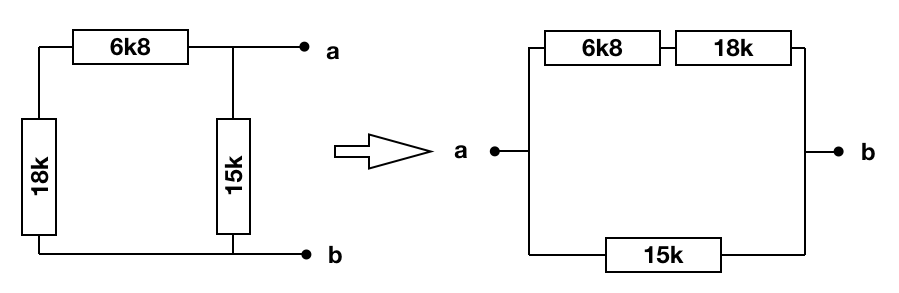
\includegraphics[width=0.7\textwidth]{Figures/32-2}
 
    Figure 3.2b: Determination of $R_{\rm Th}$
    \label{fig:32-2} 
\end{center}



\noindent so:
\begin{equation}
R_{\rm Th} = (6k8 +18k || 15k) = 9k35.
\end{equation}
 
This results in Fig. \ref{fig:32-3}c.
\begin{center}
    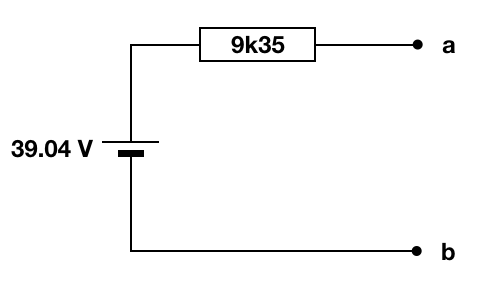
\includegraphics[width=0.5\textwidth]{Figures/32-3}
 
    Figure 3.2c: Th\'{e}venin equivalent circuit
    \label{fig:32-3} 
\end{center}

\newpage
\noindent The result in Multisim is the same (see Fig. \ref{fig:32M}d):
\begin{center}
    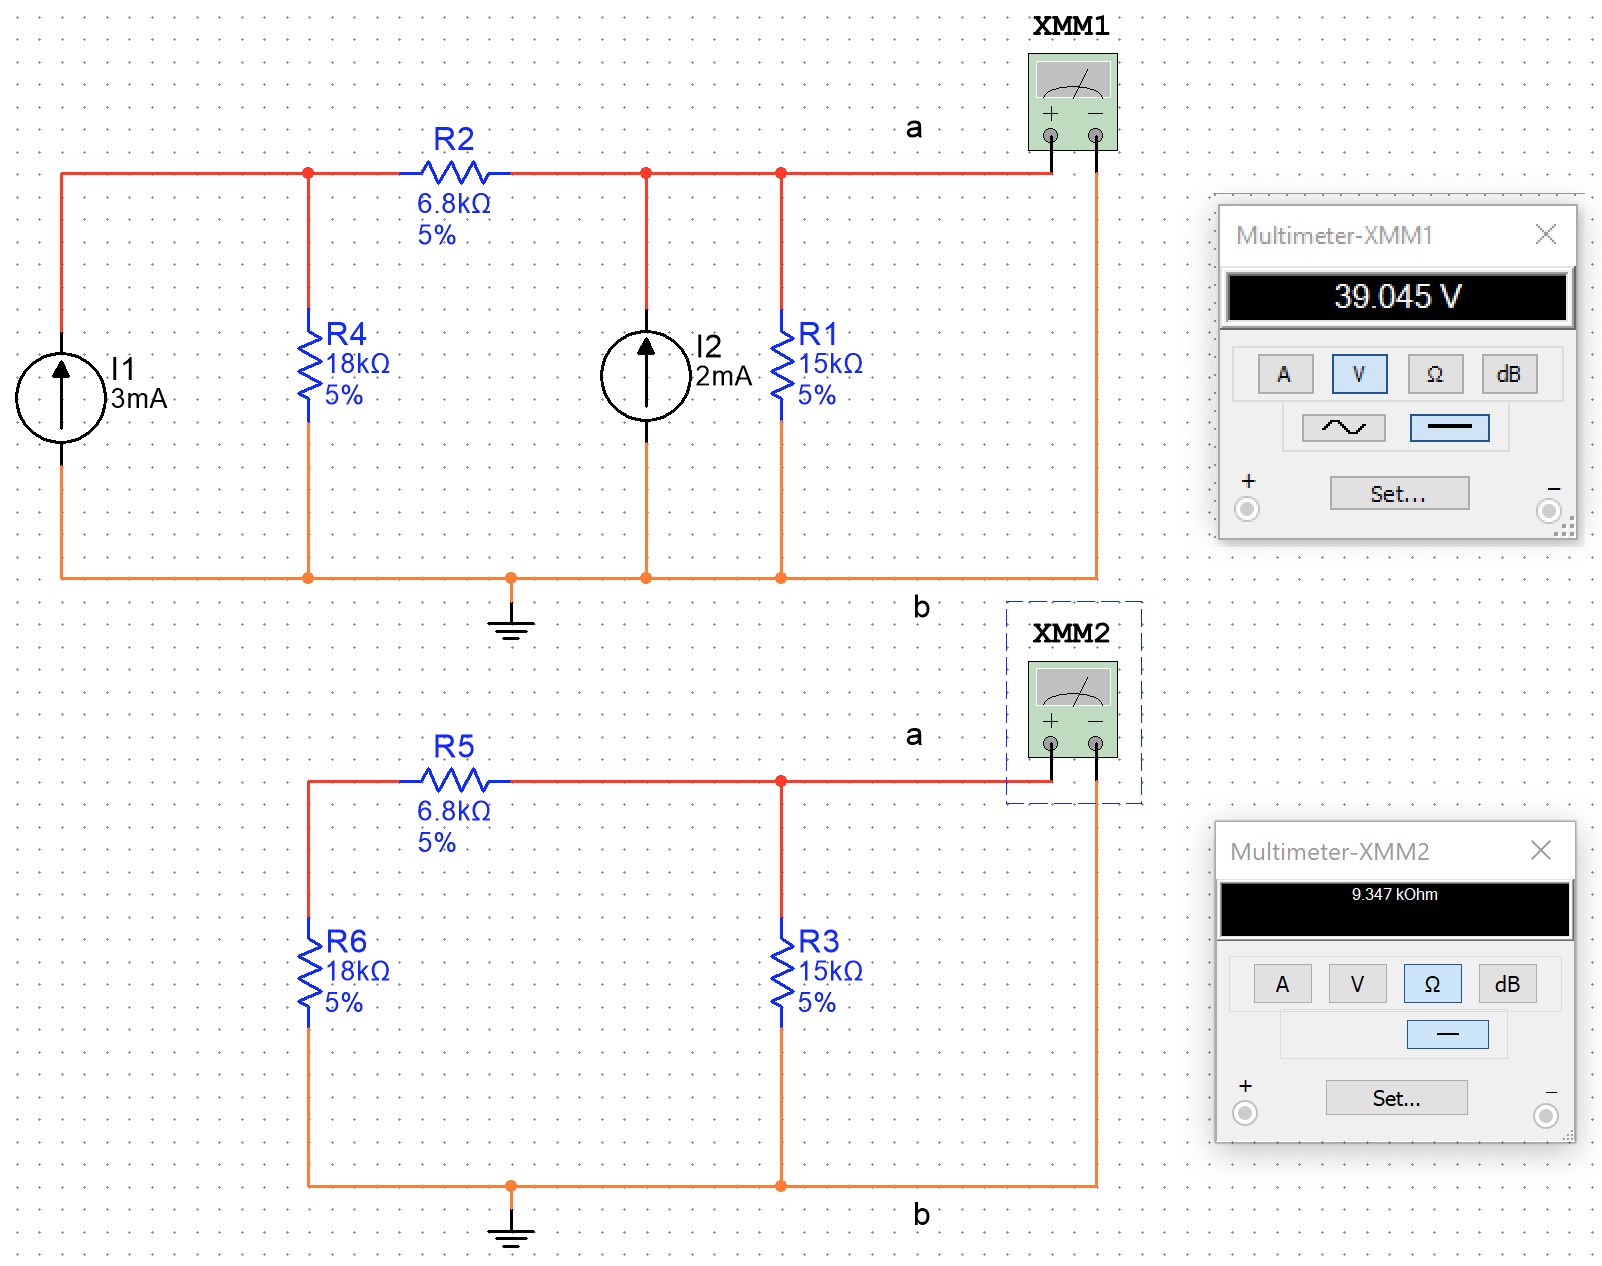
\includegraphics[width=1.0\textwidth]{Figures/32Multi}	
 
    Figure 3.2d: The results of \textit{Mult 3.2}	  
    \label{fig:32M} 
\end{center}

\newpage
\section{\textbf{Exercise 3.3}}
Fig. 3.21 
\begin{center}
    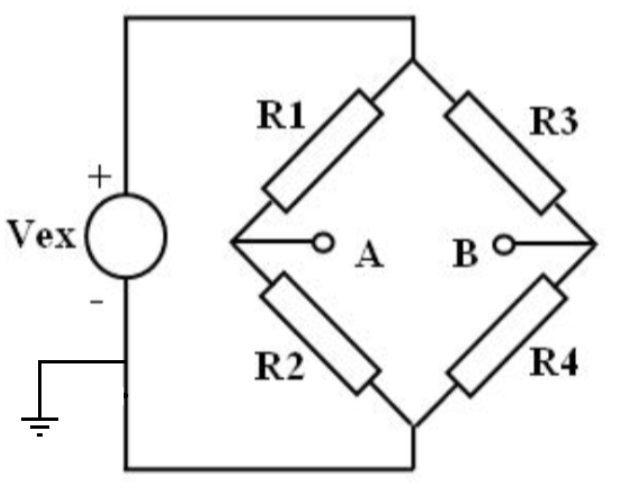
\includegraphics[width=0.4\textwidth]{Figures/33WB}	
\end{center}

\noindent in the manual tells us that
\begin{equation}
\begin{split}
V_{\rm A} & = \frac{R_1}{R_1 + R_2}V_{\rm ex}, \\
V_{\rm B} & = \frac{R_3}{R_3 + R_4}V_{\rm ex}. 
\end{split}
\end{equation}
So $V_{\rm AB}$ is given by
\begin{equation}
V_{\rm AB} = V_{\rm B} - V_{\rm A} = \left( \frac{R_3}{R_3 + R_4} - \frac{R_1}{R_1 + R_2} \right) V_{\rm ex}.
\end{equation}

This is confirmed by Multisim: with $R_2 = R_3 = R_4 = 10 \; {\rm k} \Omega$ and varying $R_1$ from 9995 to 10005 $\Omega$ results in voltage steps of 250 $\mu$V (see Fig. \ref{fig:33}). 
\begin{center}
    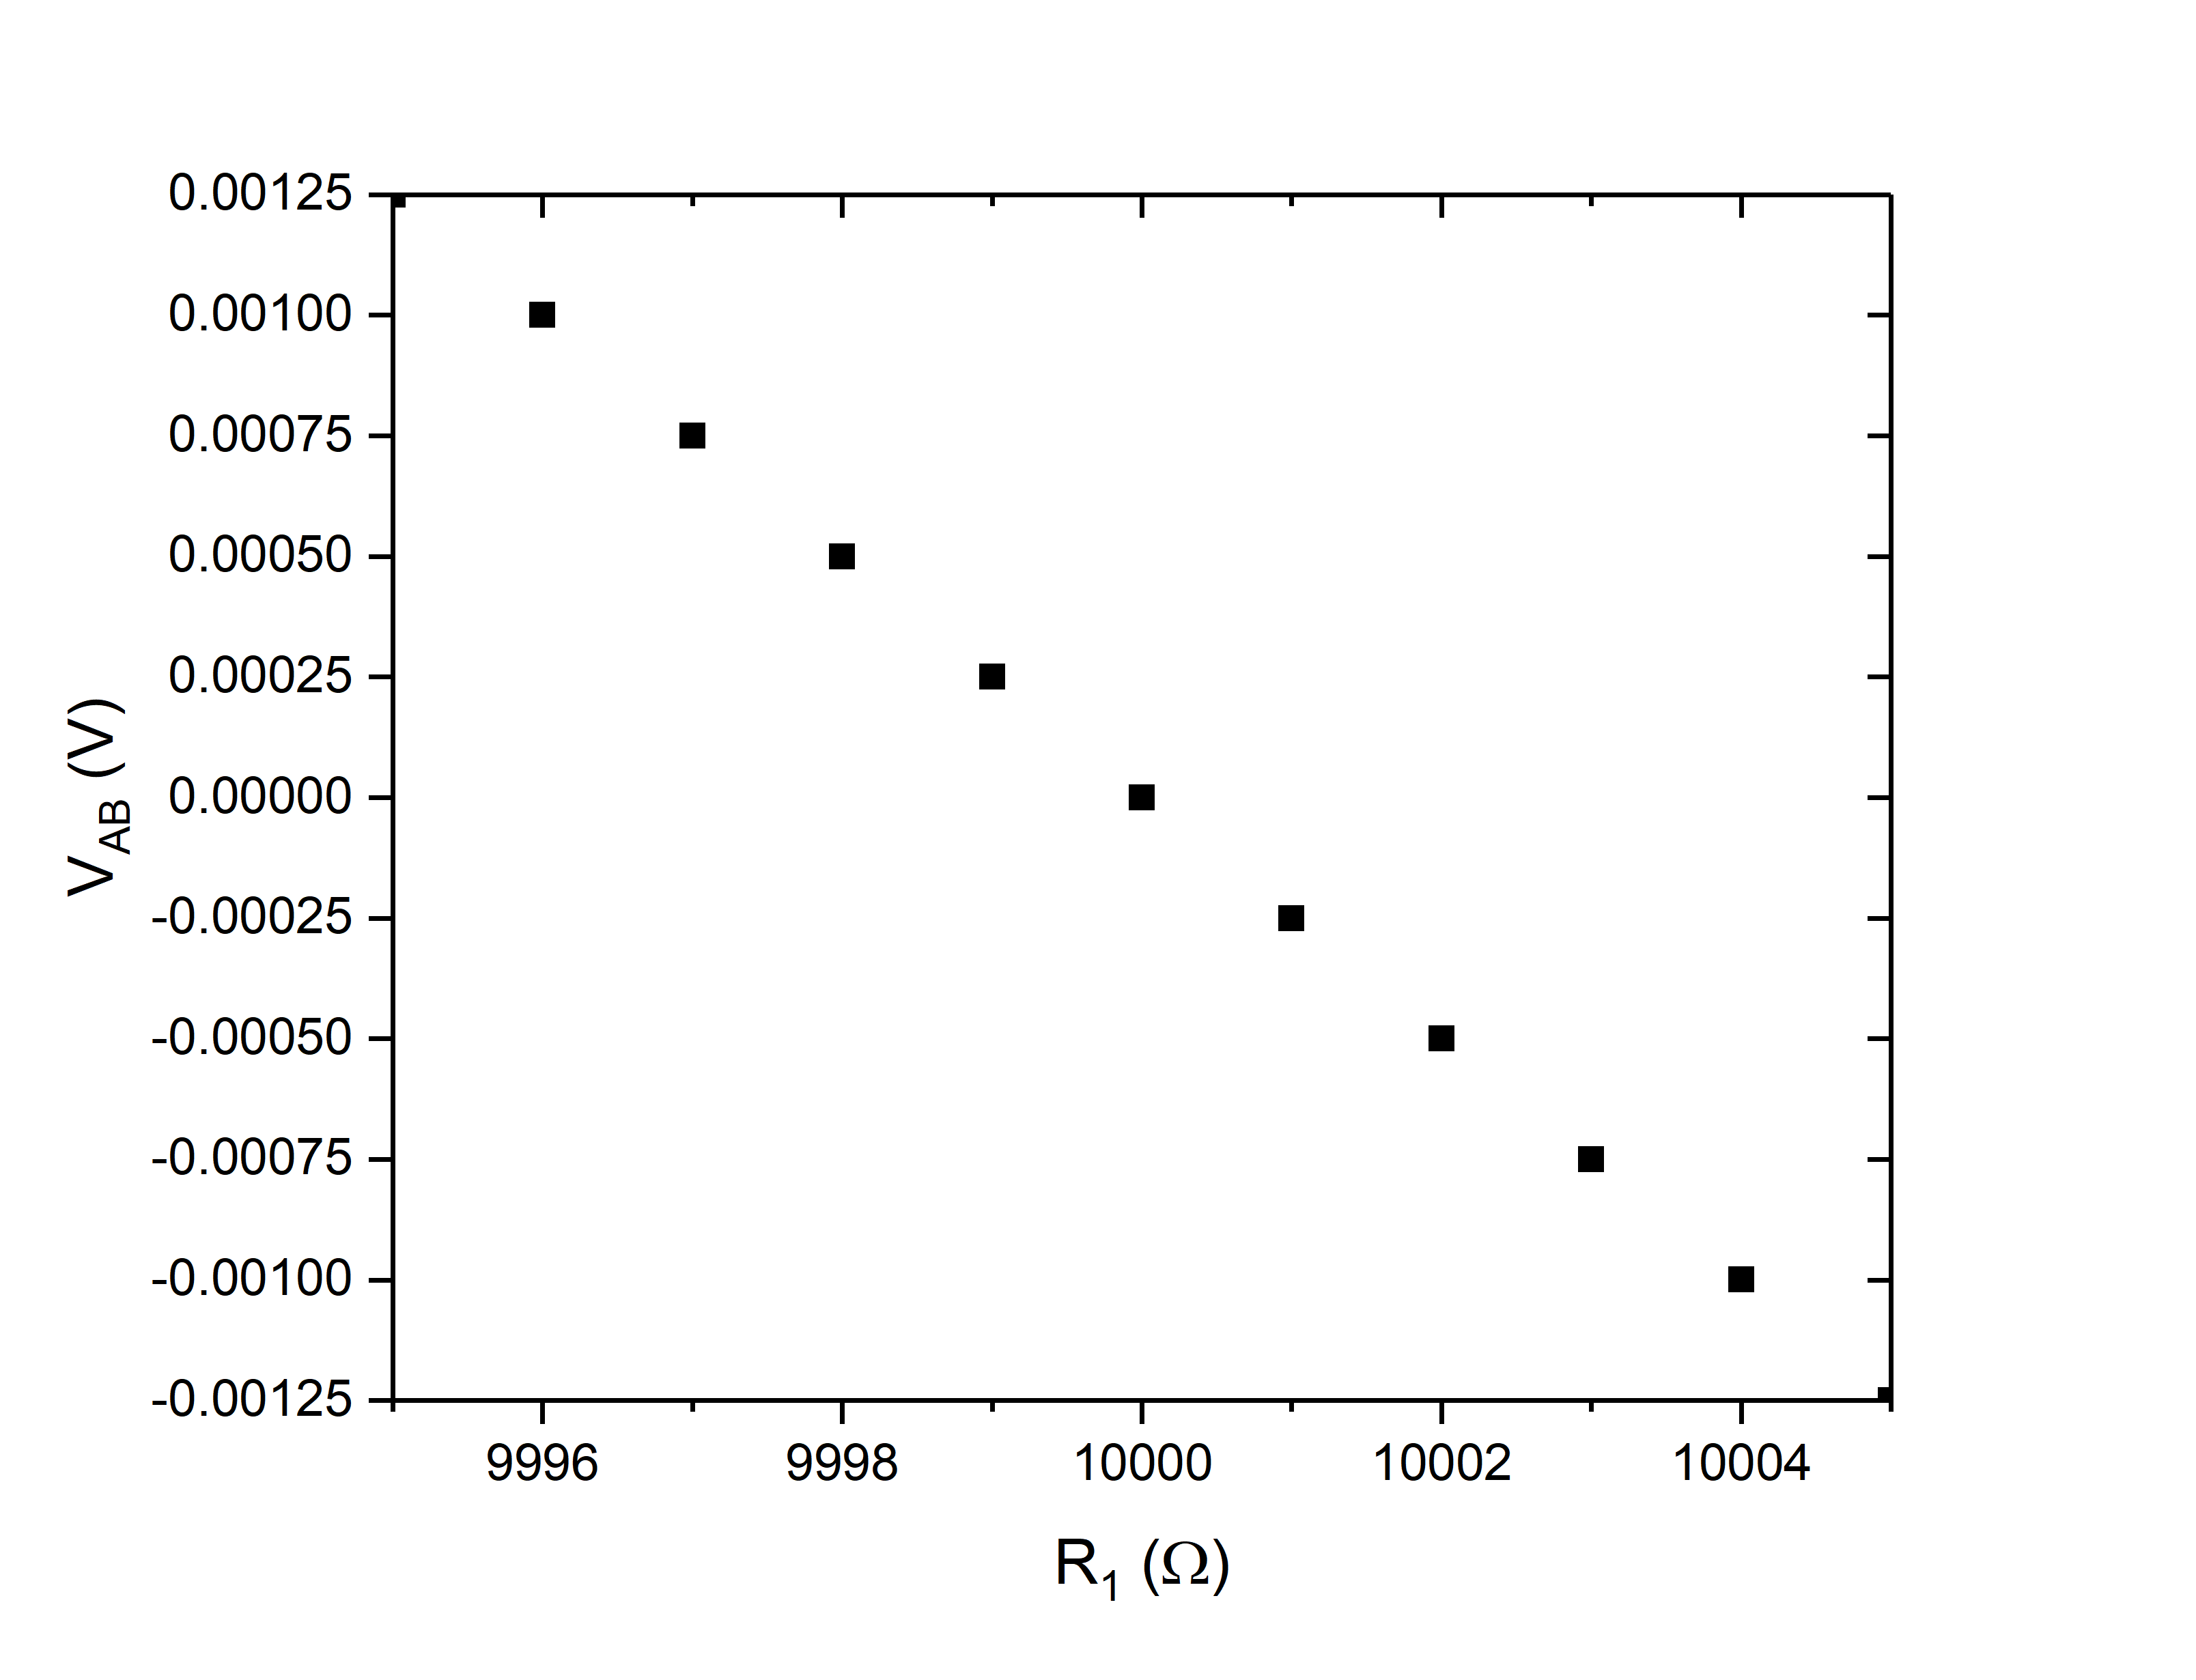
\includegraphics[width=0.7\textwidth]{Figures/33}	
 
    Figure 3.3: Results of the Wheatstone bridge  
    \label{fig:33} 
\end{center}
